% !TeX program = pdflatex
\documentclass[border=6pt]{standalone}
\usepackage{tikz}
\usetikzlibrary{arrows.meta, positioning, calc, fit, backgrounds}

\definecolor{MediumRed}{rgb}{0.925, 0.345, 0.345}
\definecolor{MediumGreen}{rgb}{0.37, 0.7, 0.66}
\definecolor{MediumBlue}{rgb}{0.015, 0.315, 0.45}
\definecolor{DarkBlue}{rgb}{0.05, 0.15, 0.35}

\begin{document}
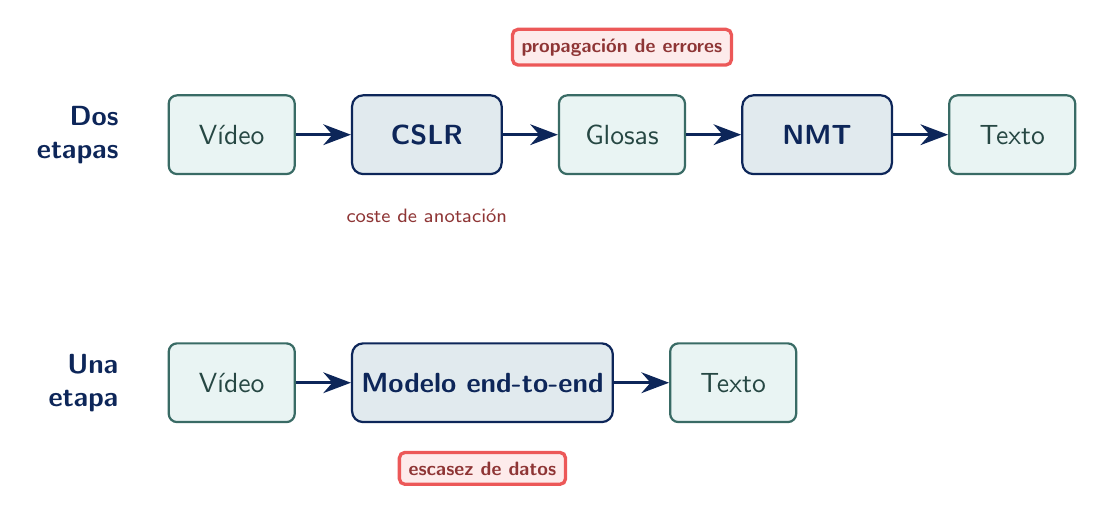
\begin{tikzpicture}[
    font=\sffamily,
    stage/.style={draw=DarkBlue, thick, rounded corners=4pt,
        fill=MediumBlue!12, text=DarkBlue, align=center,
        minimum width=1.9cm, minimum height=1.0cm},
    data/.style={draw=MediumGreen!60!black, thick, rounded corners=3pt,
        fill=MediumGreen!14, text=MediumGreen!40!black, align=center,
        minimum width=1.6cm, minimum height=1.0cm},
    flow/.style={-{Stealth[length=3.5mm]}, line width=1.2pt, DarkBlue},
]

% ============ FILA A: dos etapas (con glosas) ============
\node[data]  (a1) at (0,2.4)      {Vídeo};
\node[stage, right=0.7cm of a1] (a2) {\textbf{CSLR}};
\node[data,  right=0.7cm of a2] (a3) {Glosas};
\node[stage, right=0.7cm of a3] (a4) {\textbf{NMT}};
\node[data,  right=0.7cm of a4] (a5) {Texto};
\foreach \p/\q in {a1/a2,a2/a3,a3/a4,a4/a5} \draw[flow] (\p)--(\q);

\node[left=0.5cm of a1, text=DarkBlue, font=\sffamily\bfseries, align=right]
    {Dos\\etapas};
% cuello de botella
\node[draw=MediumRed, very thick, rounded corners=2pt, fill=MediumRed!12,
      text=MediumRed!60!black, font=\sffamily\scriptsize\bfseries,
      above=0.35cm of a3] {propagación de errores};
\node[text=MediumRed!60!black, font=\sffamily\scriptsize, below=0.3cm of a2]
    {coste de anotación};

% ============ FILA B: una etapa (sin glosas) ============
\node[data]  (b1) at (0,-0.75)     {Vídeo};
\node[stage, right=0.7cm of b1, minimum width=3.0cm] (b2) {\textbf{Modelo end-to-end}};
\node[data,  right=0.7cm of b2] (b3) {Texto};
\foreach \p/\q in {b1/b2,b2/b3} \draw[flow] (\p)--(\q);

\node[left=0.5cm of b1, text=DarkBlue, font=\sffamily\bfseries, align=right]
    {Una\\etapa};
\node[draw=MediumRed, very thick, rounded corners=2pt, fill=MediumRed!12,
      text=MediumRed!60!black, font=\sffamily\scriptsize\bfseries,
      below=0.35cm of b2] {escasez de datos};

% ============ conclusión ============
% \node[draw=MediumBlue, very thick, rounded corners=4pt, fill=MediumBlue!10,
%       text=DarkBlue, font=\sffamily\small, align=center, text width=6.4cm]
%       at (4.5,-3.0) (key)
%     {La clave no es la \textbf{cantidad} de datos,\\ sino la \textbf{estructura} que aportan las glosas.};

\end{tikzpicture}
\end{document}
